% classes
\documentclass{article}

% packages
\usepackage{graphicx}
\usepackage{fancyhdr} % Required for custom headers
\usepackage{lastpage} % Required to determine the last page for the footer
\usepackage{extramarks} % Required for headers and footers
\usepackage{courier} % Required for the courier font

\usepackage{color}
\usepackage{enumitem}

\usepackage{hyperref}

\usepackage{fancyvrb}
\newenvironment{Schunk}{}{}
\DefineVerbatimEnvironment{Sinput}{Verbatim}{fontshape=sl}

\newcommand{\code}[1]{\texttt{#1}}
% \newcommand{\pkg}[1]{\mbox{\textbf{#1}}}
\newcommand{\pkg}[1]{\mbox{\texttt{#1}}}
\newcommand{\proglang}[1]{\textsf{#1}}

% page layout

\topmargin=-0.45in
\evensidemargin=0in
\oddsidemargin=0in

\textwidth=6.5in
\textheight=9.0in

\headsep=0.25in

\linespread{1.1} % Line spacing
 
\pagestyle{fancy}

% headers and footers

\fancyhf{}

\lhead{INTR 100 Breaking Intuition}

\rhead{
\includegraphics[width=0.045\textwidth]{wmlogo.jpg}}

\cfoot{Page \thepage}


% document body

\begin{document}

\vspace*{.01mm}

\begin{center}

\Large{\textcolor{blue}{\textbf{Lab 1.}  Why William \& Mary?}}

\vspace{4mm}

\textit{Due by noon on Friday, September 11th}\\

\end{center}

\begin{figure}[h!]
\begin{center}
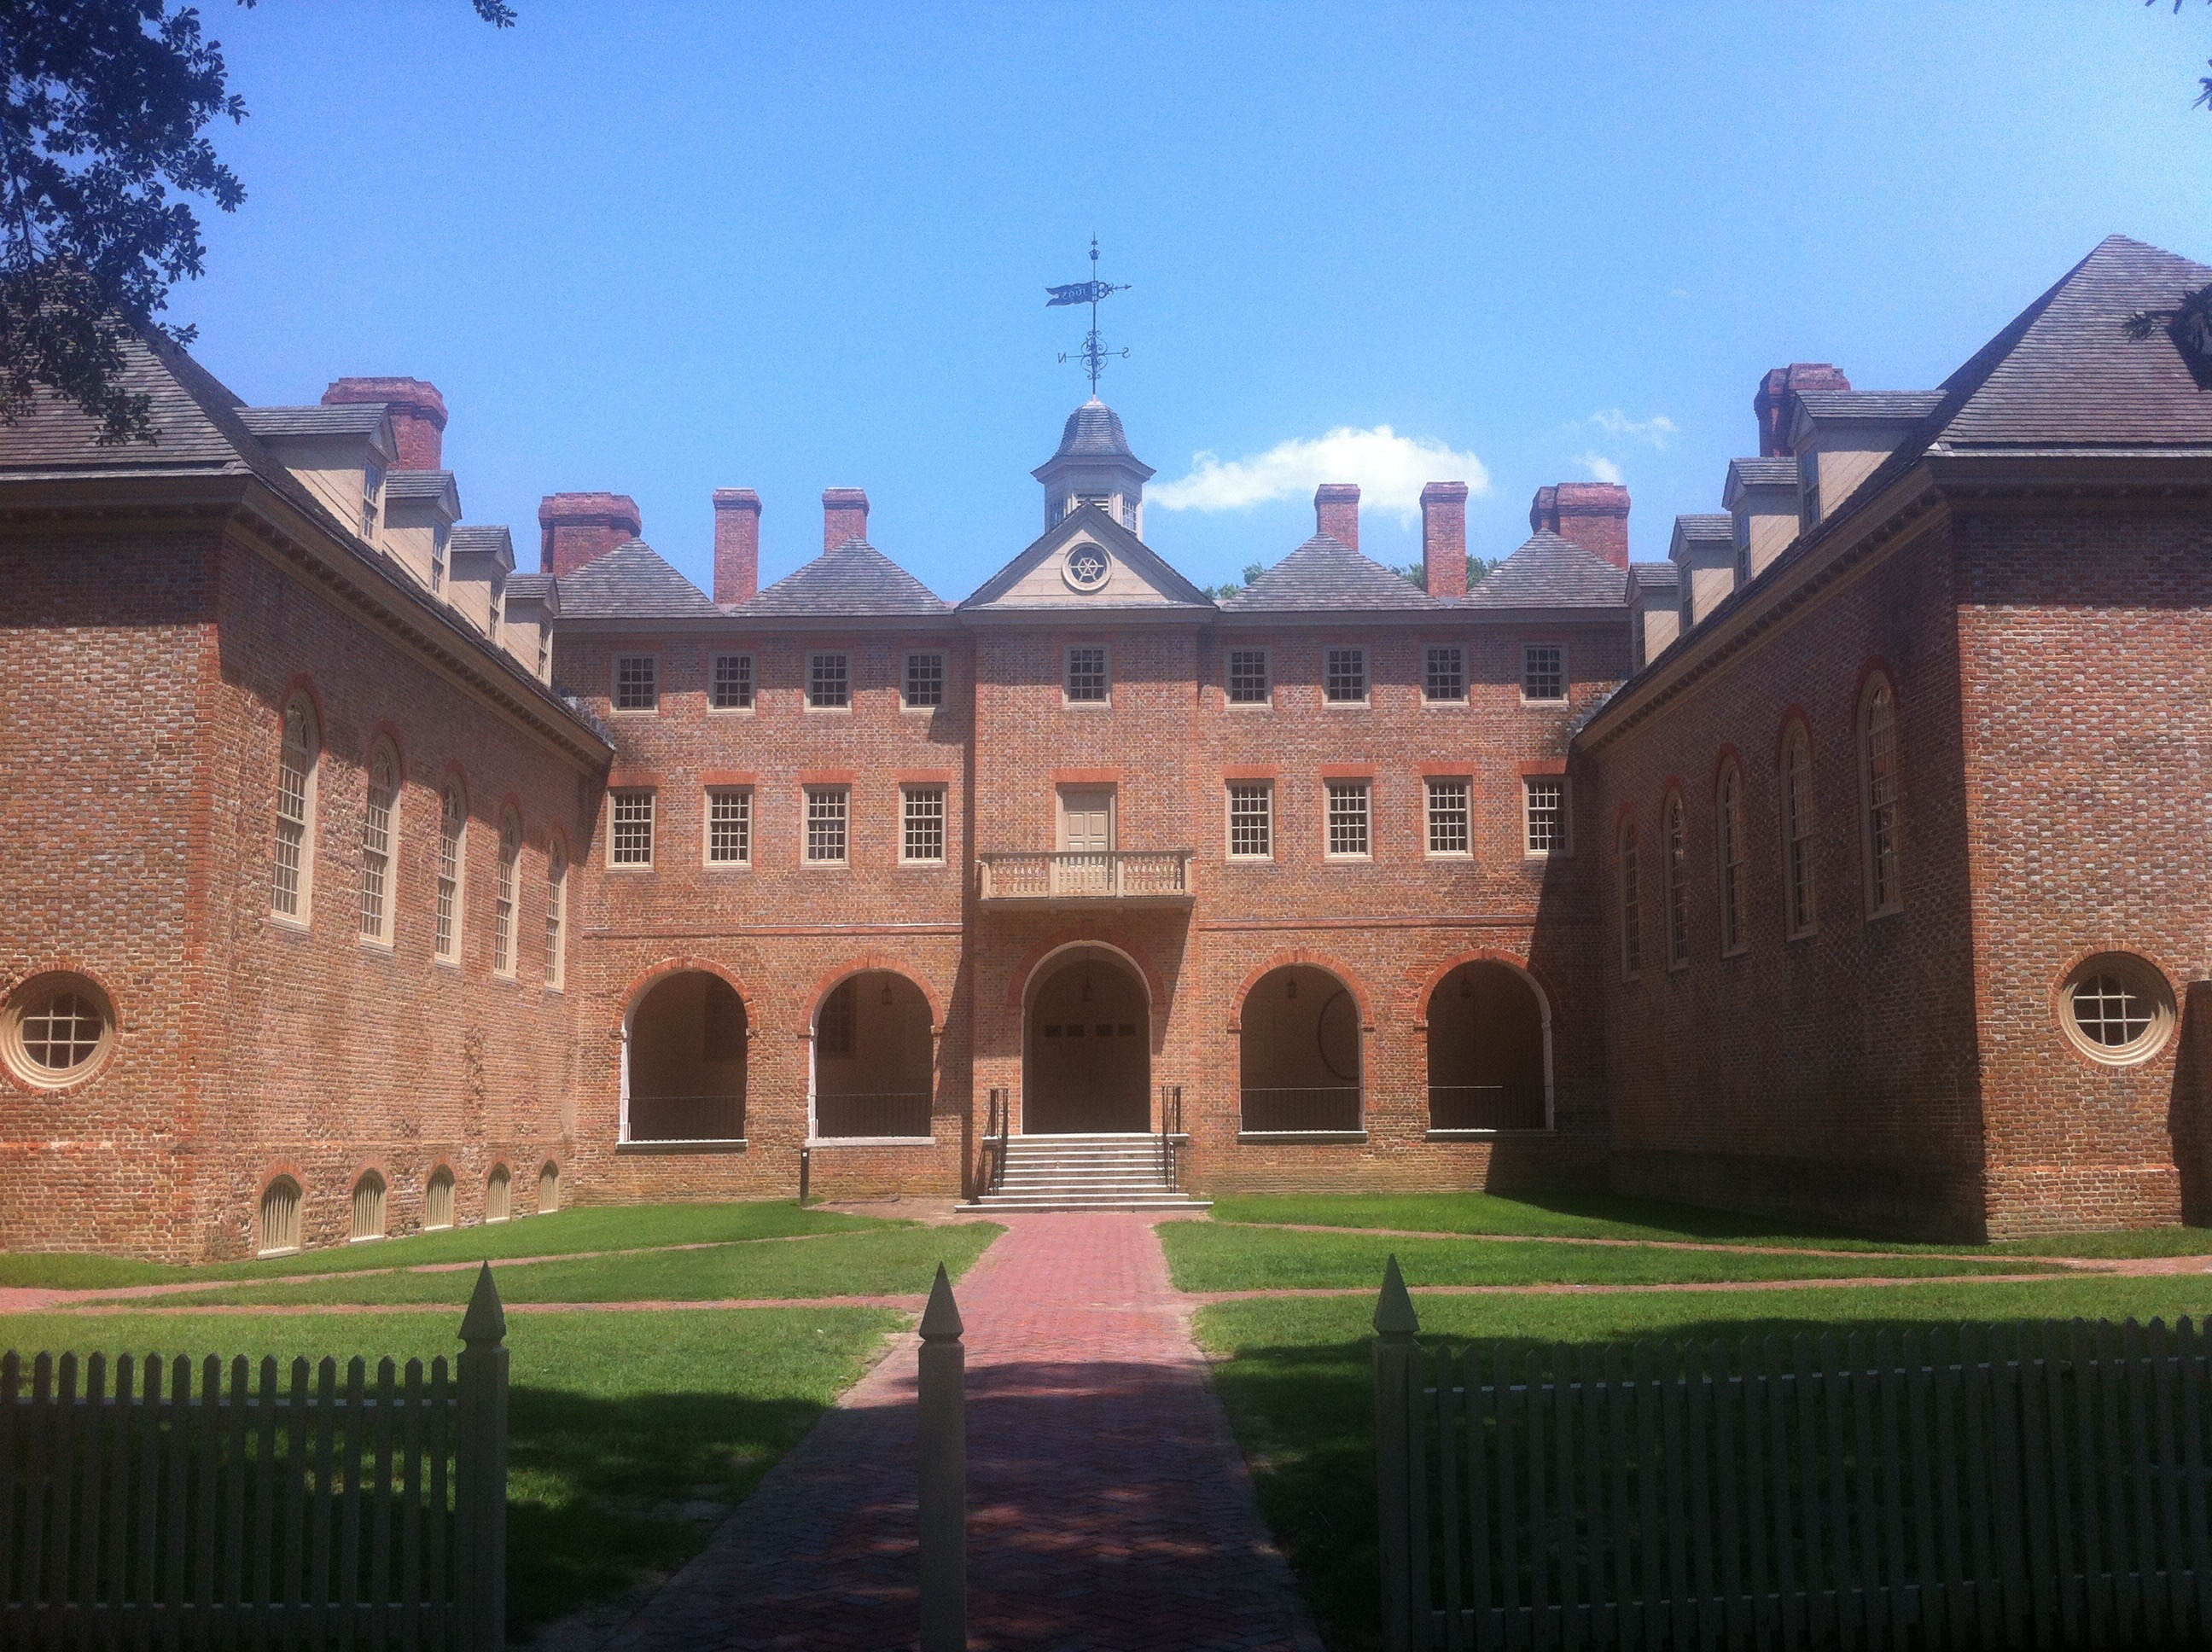
\includegraphics[width=1.0\textwidth]{wm_wrenbldg.jpg}

\end{center}
\end{figure}

\setlength{\parindent}{0cm}

\large{\textit{"I look to the diffusion of light and education as the resource most to be relied on for ameliorating the condition, promoting the virtue, and advancing the happiness of man.  %That every man shall be made virtuous, by any process whatever, is, indeed, no more to be expected, than that every tree shall be made to bear fruit, and every plant nourishment.  The brier and the bramble can never become the vine and the olive; but their asperities may be softened by culture, and their properties improved to usefulness in the order and economy of the world."}
\begin{flushright}
Letter from Thomas Jefferson to C.C. Blatchley, 1822
\end{flushright}
}

\newpage

% Enumerate the Laboratory Objectives

\large{\textbf{Laboratory in Brief:}}

\vspace{4mm}

\setlength{\leftskip}{1cm}

\setlength{\parindent}{0cm}

The purpose of this laboratory is to think about ways to justify a decision using raw, unprocessed data, while also introducing the skills you'll need to do more advanced work later in the semester. You may be asking yourself, will I really need to defend my choice to attend William and Mary for another two weeks?"  The goal of this assignment is not only to encourage you to consider in broad terms the college you have chosen and are now attending (which, by the way, was a good one), but also to begin thinking about how to obtain, manage and use data in support of this supposition.

\vspace{4mm}

\setlength{\leftskip}{0cm}

\large{\textbf{Goals of this Laboratory:}}

\begin{enumerate}[leftmargin=15mm]

\item To use "a lot more data" to explain to yourself, parents, significant other, or your best friend that William and Mary really is "the best."

\item To begin learning how to use the Statistical Computing Language \proglang{R} while also understanding how to import data to \proglang{R} from a \code{CSV} file.

\item To visualize your findings for "System 1" (we'll be learning all about this in the lecture!).

\end{enumerate}

% Enumerate the Laboratory Resources Needed

%\large{\textbf{Things to do in Preparation for this Lab:}}

%\begin{enumerate}[leftmargin=15mm]

%\item ...

%\item ...

%\item ...

%\end{enumerate}

% Step by Step Instructions for Day 1

\large{\textbf{Session 1: Monday, August 31st}}

\vspace{4mm}
\setlength{\leftskip}{1cm}
\textit{Step by Step Instructions: First we Acquire the Data}

\begin{enumerate}[leftmargin=15mm]

\item Let's download a file which gives statistics on colleges across the U.S.  In your browser go to the following address and become familiar with the National Center for Education Statistics website, which we will be using in this lab.\\ 
\url{https://nces.ed.gov/ipeds/datacenter/}

\item Find the \textbf{Download Custom Data Files} link on the left side of the webpages graphical user interface and select this button.  Once you have followed this link, you will arrive at a page that inquires \textit{"How would you like to select institutions to include in your data file/report?"}  Three options are available, but you will want to choose the link for \textbf{By Groups}.  A sub-window will appear and then also choose \textbf{EZ Group}.

\item Now you should arrive at a screen that asks for more detail about which institutions you want to select from the database.  Select the  \textbf{U.S. only button} and then the Search button (there were 7597 at the time I did the search).  The screen should appear like this. 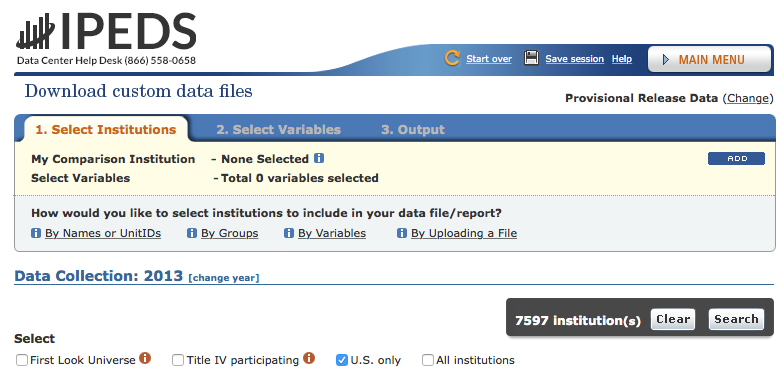
\includegraphics[width=0.75\textwidth]{us_only.png}

\item On the next page, look for the \textbf{Continue button} which is located below the \textbf{Download custom data files} box and after the statement \textit{When you have finished selecting institutions} 
\includegraphics[width=0.1\textwidth]{continue.png} to Step 2 - Select Variables.

\item On the following page you will begin selecting the individual variables that will be used in your analysis.  First find the \textbf{Frequently used/Derived variables} tab and expand that under \textbf{Institutions} until you see several check mark boxes that selection.  Choose \textbf{State abbreviation}. 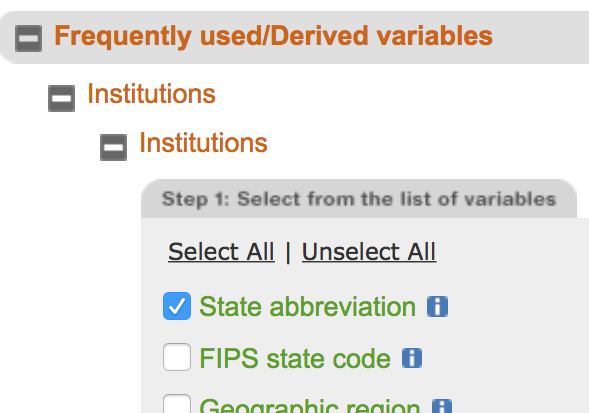
\includegraphics[width=0.35\textwidth]{state.png} Then under \textbf{Total cost of attendance} and \textbf{price} select the check boxes for the first four annual sets of \textbf{Tuition and fees}. 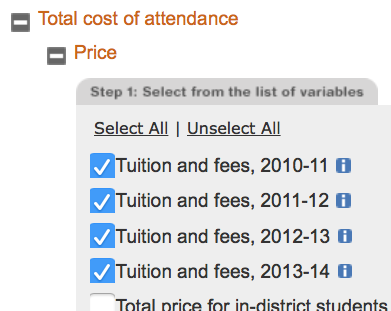
\includegraphics[width=0.35\textwidth]{cost.png}  Next click on the \textbf{Revenues and expenditures: Fiscal year 2013} and choose the \textbf{Expenses for salaries, wages and nbenefits as a percent of total expenses, by function}.  Finally, check the first four boxes: \textbf{core expenses, instruction, research and public service}. 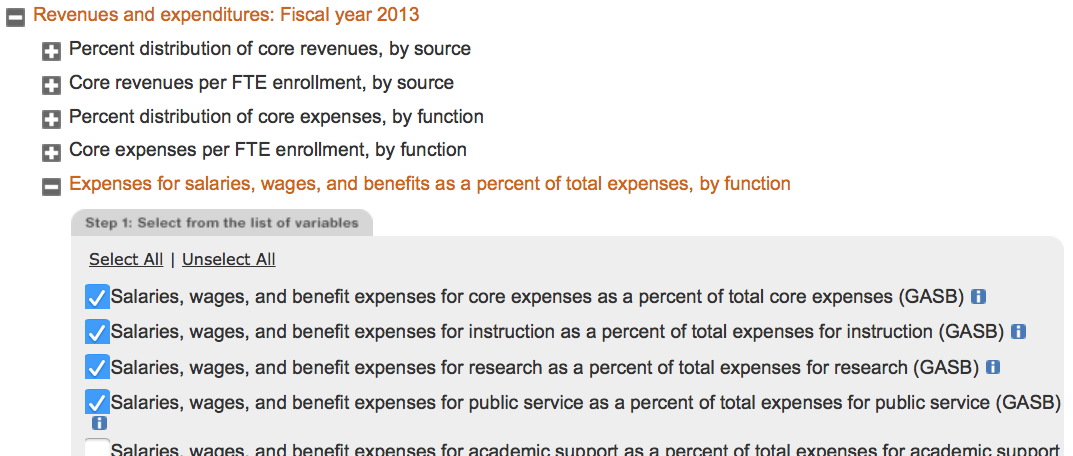
\includegraphics[width=0.7\textwidth]{core.png}

\item Keep in mind that for this stage of the lab we will walk you through one very specific analysis, but to get the maximum grade on this assignment you will need to download more data to make your own case, so you may want to choose one or two additional variables you think are interesting now.

\item Finally, scroll back up to the top and click 
\includegraphics[width=0.125\textwidth]{continue2.png} , then under the headline bar \textbf{Year 2013} download your data as a CSV. 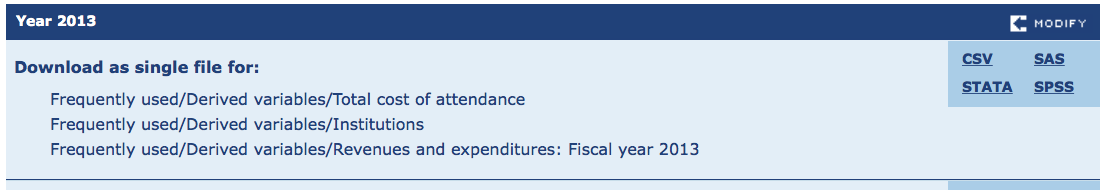
\includegraphics[width=0.5\textwidth]{csv.png}


\vspace{4mm}
\setlength{\leftskip}{0cm}
\textit{Now We Import the Data to R}

\item Open \proglang{R} or R Studio

\item Identify where the console is the programming interface.  It should look something like the following.  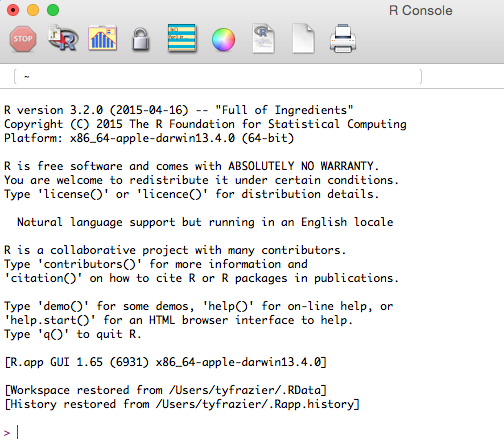
\includegraphics[width=0.5\textwidth]{console.png}  Go ahead try entering a few commands.  Try entering the following commands in the R console.  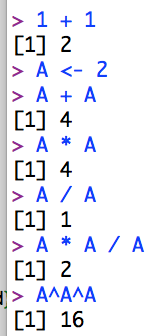
\includegraphics[width=0.2\textwidth]{A.png}

\item Now lets create a script file.  In the R user interface find the drop down menu for \textbf{file} and choose \textbf{New Document}.  Creating a script file enables us to do two things.  First we can save our code and reuse it later.  Second can use our script document as the source of which commands we will send to the console for execution.  Go ahead and write the same code in your script file from item 9 and then use the \textbf{command enter} key combination in order to send those commands to the console. 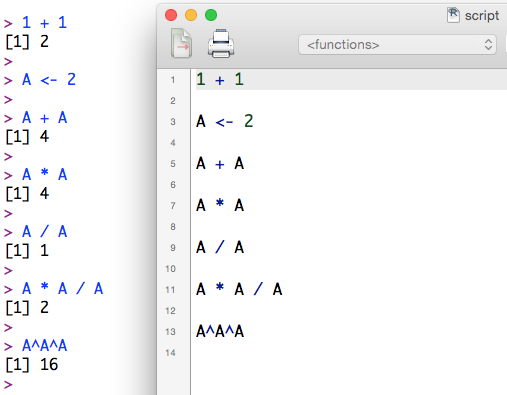
\includegraphics[width=0.85\textwidth]{script.png} Be sure to save the file and give it a name.  I recommend just calling it "lab1.csv" in order to keep it simple.  Using your William \& Mary "H" drive is a good idea.

\item Since now you have some basics under your belt, lets go ahead and load the \code{CSV} file/folder we downloaded from the National Center for Education Statistics.  First copy the file into your William \& Mary \code{H:\textbackslash\textbackslash} drive so it doesn't get deleted.  To do this, open up "My Computer", go to "Downloads", and copy the file you downloaded (click on it and push "ctrl+c").  Now, go back to My Computer, choose your H drive, and paste it (ctrl+v on your keyboard).  While in this case, you probably won't have to work with zip files, in the future you will likely need to learn how to extract files from a zip.  I recommend you google "how to extract a zip file" if you need help, but you can also raise your hand to ask an instructor or TA.  This stuff can get complicated, so never hesitate to ask if you get lost!

\item Back in \proglang{R}, in the window at the top, type in the following commands below.

\begin{Schunk}
\begin{Sinput}

R> setwd("H:\textbackslash\textbackslash")

R> collegeData \textless - read.csv("lab1.csv")

R> view(collegeData)

R> str(collegeData)

R> names(collegeData)

R> dim(collegeData)

R> nrow(collegeData)

\end{Sinput}
\end{Schunk}

\item Click on each line and then click "run" like we did before to see each line in action, or select the entire script and click "run" to run it all at once.

\end{enumerate}

% Step by Step Instructions for Day 2

\setlength{\leftskip}{0cm}

\large{\textbf{Session 2: Wednesday, September 2nd}}

\vspace{4mm}
\setlength{\leftskip}{1cm}
\textit{Step by Step Instructions:}

\begin{enumerate}[leftmargin=15mm]

\item For starting out on day 2, let's actually run a some analysis in \proglang{R}.  For example, let us consider the question, how many colleges are in each state?  When you type in \code{names(collegeData)}, you'll notice one of the names is \code{HD2013.State.abbreviation} - one of the columns you requested when you did the download.  To see how many colleges are in each state, type in:

\begin{Schunk}
\begin{Sinput}
R> table(collegeData$HD2013.State.abbreviation)
\end{Sinput}
\end{Schunk}

\item Now, let's use a different command to identify the average tuition across all colleges:?
\begin{Schunk}
\begin{Sinput}
R> summary(collegeData$DRVIC2013.Tuition.and.fees..2013.14)
\end{Sinput}
\end{Schunk}

\item We can also do the same thing, but only looking at Virginia schools ? does Virginia have a higher average tuition or lower than the rest of the country?:

\begin{Schunk}
\begin{Sinput}
R> VA_colleges <- collegeData[which(collegeData$HD2013.State.abbreviation=="Virginia"),]
R> summary(VA_colleges$DRVIC2013.Tuition.and.fees..2013.14)
\end{Sinput}
\end{Schunk}

\item What if we want to get really clever, and identify only those institutions in VA that are above the national mean?  Is William and Mary above the national mean?

\begin{Schunk}
\begin{Sinput}
R> AboveUSMeanVA <- collegeData[which(collegeData$HD2013.State.abbreviation=="Virginia" & collegeData$DRVIC2013.Tuition.and.fees..2013.14 > 14140),]
R> View(AboveUSMeanVA)
\end{Sinput}
\end{Schunk}

\item You can read through each entry to figure out what William and Mary's tuition is, or you could type this:

\begin{Schunk}
\begin{Sinput}
R> collegeData[which(collegeData$institution.name=="College of William and Mary"),]$DRVIC2013.Tuition.and.fees..2013.14
\end{Sinput}
\end{Schunk}

\item You can use similar approaches to find the cheapest and most expensive schools in the country:

\begin{Schunk}
\begin{Sinput}
R> min(collegeData$DRVIC2013.Tuition.and.fees..2013.14, na.rm=TRUE)?R> max(collegeData$DRVIC2013.Tuition.and.fees..2013.14, na.rm=TRUE)?R> minColCost <- min(collegeData$DRVIC2013.Tuition.and.fees..2013.14, na.rm=TRUE)?R> maxColCost <- max(collegeData$DRVIC2013.Tuition.and.fees..2013.14, na.rm=TRUE)?R> collegeData[which(collegeData$DRVIC2013.Tuition.and.fees..2013.14 == minColCost),]$institution.name?R> collegeData[which(collegeData$DRVIC2013.Tuition.and.fees..2013.14 == maxColCost),]$institution.name
\end{Sinput}
\end{Schunk}

\vspace{4mm}
\setlength{\leftskip}{0cm}
\textit{Analysis}

\item Now, we're going to do some basic analysis that you can include on your revised infographic.  Note the goal of this \proglang{R} tutorial is not to create beautiful visualisations ? though \proglang{R} can do that.  Rather, we want to extract data you can then use in visme to improve your original infographic.  Let's do something very simple to start: how does the percentage increase of William and Mary's tuition compare to (a) all schools, and (b) Virginia schools from 2010 to the 2013-2014 school year?

\item First, let's calculate this for William and Mary (type in WMchange) at the end.

\begin{Schunk}
\begin{Sinput}
R> WMTuition_2014 <- collegeData[which(collegeData$institution.name=="College of William and Mary"),]$DRVIC2013.Tuition.and.fees..2013.14?R> WMTuition_2010 <- collegeData[which(collegeData$institution.name=="College of William and Mary"),]$DRVIC2013.Tuition.and.fees..2010.11
R> WM_change <- WMTuition_2014 / WMTuition_2010
\end{Sinput}
\end{Schunk}

\item Now, let's calculate the average change for every other school.  This is the first time we're going to add our own new ?column? to the data frame.  To see how this works, first type in the below command, which will show you the current set of columns (i.e., the data available for each college):?
\begin{Schunk}
\begin{Sinput}
R> names(collegeData)
\end{Sinput}
\end{Schunk}

\item Now, let's create a new one that tells us how much tuition has changed.  Note this is the same thing we did for just William and Mary, but for every school:

\begin{Schunk}
\begin{Sinput}
R> collegeData$All_change <- collegeData$DRVIC2013.Tuition.and.fees..2013.14 / collegeData$DRVIC2013.Tuition.and.fees..2010.11
R> names(collegeData)
\end{Sinput}
\end{Schunk}

\item Note now there is a new "name" in collegeData, which represents a new column.  Let's summarize the change column now:

\begin{Schunk}
\begin{Sinput}
R> summary(collegeData$All_change)
\end{Sinput}
\end{Schunk}

\item Let's do a comparison between the tuition in 2014 and the percent of that money spent on instructors salary.  First, let's look it up for William and Mary:

\begin{Schunk}
\begin{Sinput}
R> collegeData[which(collegeData$institution.name=="College of William and Mary"),]$DRVF2013.Salaries..wages..and.benefit.expenses.for.instruction.as.a.percent.of.total.expenses.for.instruction..GASB.
\end{Sinput}
\end{Schunk}

\item And second, let's compare that to the national average:

\begin{Schunk}
\begin{Sinput}
R> summary(collegeData$DRVF2013.Salaries..wages..and.benefit.expenses.for.instruction.as.a.percent.of.total.expenses.for.instruction..GASB.)
\end{Sinput}
\end{Schunk}

\item Finally, let's plot out all schools tuition in 2014 contrasted to the \% of tuition they spend on instructors salary.

\begin{Schunk}
\begin{Sinput}
R> plot(collegeData$DRVF2013.Salaries..wages..and.benefit.expenses.for.instruction.as.a.percent.of.total.expenses.for.instruction..GASB., collegeData$DRVIC2013.Tuition.and.fees..2010.11)
\end{Sinput}
\end{Schunk}

\item That on it's own isn't particularly helpful, as it's hard to see patterns with outliers and without knowing which dot is William and Mary.  It's also probably more fair to compare to only Virginia schools, so let's drop out everything that isn't Virginia and label W\&M in an appropriate color.  First, re-use the old VAcolleges dataset you made:

\begin{Schunk}
\begin{Sinput}
R> plot(VA_colleges$DRVF2013.Salaries..wages..and.benefit.expenses.for.instruction.as.a.percent.of.total.expenses.for.instruction..GASB., VA_colleges$DRVIC2013.Tuition.and.fees..2010.11)
\end{Sinput}
\end{Schunk}

\item Now, let's label just W\&M ? save this figure (click the ?export? button above the chart) as you will be turning it in!

\begin{Schunk}
\begin{Sinput}
R> WM_plot <- collegeData[which(collegeData$institution.name=="College of William and Mary"),]
points(WM_plot$DRVF2013.Salaries..wages..and.benefit.expenses.for.instruction.as.a.percent.of.total.expenses.for.instruction..GASB., WM_plot$DRVIC2013.Tuition.and.fees..2010.11, col="green")
\end{Sinput}
\end{Schunk}

\end{enumerate}

% Step by Step Instructions for Day 3

\setlength{\leftskip}{0cm}

\large{\textbf{Session 3: Monday, September 7th}}

\vspace{4mm}
\setlength{\leftskip}{1cm}
\textit{Step by Step Instructions:}

\begin{enumerate}[leftmargin=15mm]

\item Go back to Step 1 from Session 1 and choose at least one variable that was not included in this analysis.  Follow all the steps from Session 1. 

\item Conduct similar analysis from Session 2, plot your variable and save the output. 

\end{enumerate}

% Step by Step Instructions for Day 4

\setlength{\leftskip}{0cm}
 
\large{\textbf{Session 4: Wednesday, September 9th}}

\vspace{4mm}
\setlength{\leftskip}{1cm}
\textit{Step by Step Instructions: Lab Questions}

\begin{enumerate}[leftmargin=15mm]

\item Calculate which two states have the most colleges, and how many does each one have?

\item Calculate the mean tuition cost for the US and for Virginia?  Does Virginia have a higher or lower average tuition cost than the rest of the USA?  What is this difference?

\item Calculate the 2010-2011, 2011-2012, 2012-2013, and 2013-2014 Tuition and Annual Percent Change for William \& Mary, all Universities in Virginia, and all Universities in the USA.

\item Create a graph showing USD invested in instruction as compared with tuition costs and highlight William \& Mary.  Create a similar chart considering the mean of these two values for all Universities in Virginia and all Universities in the USA.

\item Calculate what are the most and least expensive Universities in Virginia and the USA. 

\item Attach a printed copy of your "visme" visualisation to this document, or submit it electronically.  What variable did you include that was not explicitly a part of this lab?  What challenges did you have in retrieving it, and how did you use it to illustrate William and Mary is an exceptional (or, crazy!) choice of where to get your degree?

\end{enumerate}


\vspace{4mm}
\setlength{\leftskip}{0cm}
\textit{Stretch Goals}

Made it this far?  Want to try to go even farther?  Just want to learn?  Try any of the following to really impress us, it won't count for your grade, but it'll give you a leg up on future assignments:
\begin{itemize}
\item In your download, ask for the "latitude" and "longitude" columns, then plot colleges following this tutorial: \url{http://www.milanor.net/blog/?p=594}
\item Examine how US schools compare to international schools.
\item Make similar comparisons with a different dataset ? i.e., try
\end{itemize}


% Final Output from Laboratory

\setlength{\leftskip}{0cm}

\large{\textbf{Final Output for Submission}}

\vspace{4mm}
\setlength{\leftskip}{1cm}
\textit{Due by noon on Friday, November 13th:}
\vspace{2mm}

...  Make certain the Final Report meets the following criteria.

\begin{itemize}

\item Single spaced with block paragraph style and 10 to 12 font, preferably New Times Roman, Arial, Courier or a similar font.
\item x to x pages in length
\item Output from Session 2
\item Output from Session 3
\item Answers to Questions Considered during Session 4

\end{itemize}

% Grading

\setlength{\leftskip}{0cm}

\textbf{Grading}

\vspace{4mm}

\setlength{\leftskip}{1cm}

\setlength{\parindent}{0cm}

This lab will be graded based on the six deliverables identified on the final page of this lab.  The first five questions are worth 50\% of your grade, and are based on your capability to work through the steps below (i.e., if you follow the steps, you'll get the right answer!).  The last question ? question 6 ? asks you to update your visualisation you created last week using not only the datasets referenced in this lab, but asks you to download at least one additional variable to use in your update.  The process of critically deciding what data to use, how to analyse it, and how to visualise it will be worth the remaining 50\% of your grade.
%----------------------------------------------------------------------------------------

\end{document}